
% Cal Poly Thesis
% 
% based on UC Thesis format
%
% modified by Mark Barry 2/07.
%




\documentclass[12pt]{ucthesis}

%\newif\ifpdf
%\ifx\pdfoutput\undefined
%    \pdffalse % we are not running PDFLaTeX
%\else
%\pdfoutput=1 % we are running PDFLaTeX
%\pdftrue \fi

\usepackage{url}
%\ifpdf

    \usepackage[pdftex]{graphicx}
    % Update title and author below...
    \usepackage[pdftex,plainpages=false,breaklinks=true,colorlinks=true,urlcolor=blue,citecolor=blue,%
                                       linkcolor=blue,bookmarks=true,bookmarksopen=true,%
                                       bookmarksopenlevel=3,pdfstartview=FitV,
                                       pdfauthor=Christopher Gibson,
                                       pdftitle=An Approach to Point-Based Color bleeding With Volumes,
                                       pdfkeywords={thesis, masters, cal poly, volume rendering, global illumination}
                                       ]{hyperref}
    %Options with pdfstartview are FitV, FitB and FitH
    \pdfcompresslevel=1

%\else
%    \usepackage{graphicx}
%\fi

\usepackage{amssymb}
\usepackage{amsmath}
\usepackage[letterpaper]{geometry}
\usepackage[overload]{textcase}



%%%%%\bibliographystyle{abbrv}

\setlength{\parindent}{0.25in} \setlength{\parskip}{6pt}

\geometry{verbose,nohead,tmargin=1.25in,bmargin=1in,lmargin=1.5in,rmargin=1.3in}

\setcounter{tocdepth}{2}


% Different font in captions (single-spaced, bold) ------------
\newcommand{\captionfonts}{\small\bf\ssp}

\makeatletter  % Allow the use of @ in command names
\long\def\@makecaption#1#2{%
  \vskip\abovecaptionskip
  \sbox\@tempboxa{{\captionfonts #1: #2}}%
  \ifdim \wd\@tempboxa >\hsize
    {\captionfonts #1: #2\par}
  \else
    \hbox to\hsize{\hfil\box\@tempboxa\hfil}%
  \fi
  \vskip\belowcaptionskip}
\makeatother   % Cancel the effect of \makeatletter
% ---------------------------------------

\begin{document}

% Declarations for Front Matter

% Update fields below!
\title{An Approach to Point-Based Color bleeding With Volumes}
\author{Christopher Gibson}
\degreemonth{June} \degreeyear{2011} \degree{Master of Science}
\defensemonth{June} \defenseyear{2011}
\numberofmembers{3} \chair{Zo\"{e} Wood, Ph.D.} \othermemberA{Aaron Keen, Ph.D.} \othermemberB{Chris Lupo, Ph.D.} \field{Computer Science} \campus{San Luis Obispo}
\copyrightyears{seven}



\maketitle

\begin{frontmatter}

% Custom made for Cal Poly (by Mark Barry, modified by Andrew Tsui).
\copyrightpage

% Custom made for Cal Poly (by Andrew Tsui).
\committeemembershippage

\begin{abstract}

Achieving realistic or believable global illumination in scenes with participating media is expensive.  Light interacts with the particles of a volume, creating complex radiance patterns.  This paper introduces an extension to the commonly used point-based color bleeding technique which allows fast, believable in- and out-scattering building on existing data structures and paradigms.  The proposed method achieves results comparable to those produced with Monte Carlo ray tracing but with drastically reduced run times, speeding up renders by around 8 times. 

\end{abstract}

%\begin{acknowledgements}

%   Thank you...

%\end{acknowledgements}


\tableofcontents


\listoftables

\listoffigures

\end{frontmatter}

\pagestyle{plain}




\renewcommand{\baselinestretch}{1.66}


% ------------- Main chapters here --------------------





\chapter{Introduction}
\label{intro}

The ability to render scenes with realistic lighting is desirable for many entertainment application settings such as film.  Great results have been achieved for large scenes using point based color bleeding~\cite{christensen:2008} algorithms.  These algorithms, however, tend to limit or omit entirely the lighting contribution from volumetric data or participating media within the scenes.  This paper presents an algorithm to address this missing component in the point based color bleeding algorithm.  Specifically, we propose the addition of a data representation tuned to volumes,  \emph{light-voxel (or lvoxel)} to address the need to represent participating media to an existing global illumination algorithm which leverages a point cloud representation of a scene.  

  The proposed method achieves results comparable to those produced with Monte Carlo ray tracing but with drastically reduced run times, speeding up renders by around 8 times.  Figure~\ref{fig:compare} illustrates a comparison of our algorithm and Monte Carlo ray traced results.

\begin{figure}[h!]
    \centering
    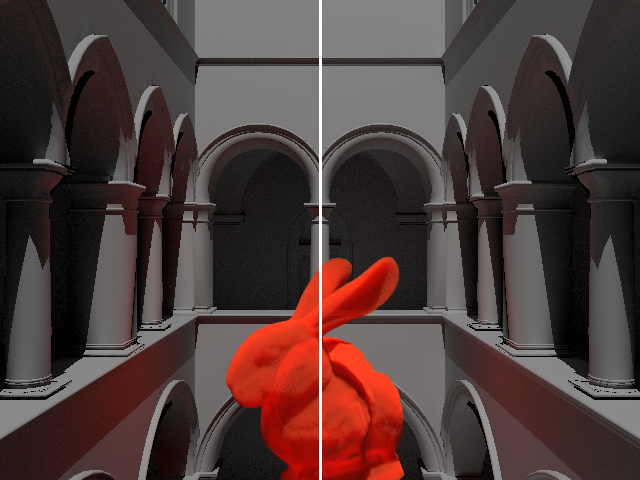
\includegraphics[width=80mm]{img/compare.png}
    \caption{Comparison of the PCB extension (left) and traditional Monte Carlo results (right.)}
    \label{fig:compare}
\end{figure}



\chapter{Background}
\label{background}

The goal of the proposed method is to include volumetric representations into a global illumination algorithm in a fast and coherent way. One of the unique features of participating media is that they must be represented with a more complex data-structure than solid geometric objects which are usually polygonalized in most rendering processes.  Light interacts with the particles of a volume, creating complex radiance patterns (increasing the necessary computational complexity exponentially.) In particular the most fundamental concepts are presented here,  (based off of  \cite{pbrt}).



%----------------------------------%
\section{Radiance}

\begin{figure}[h!]
    \centering
    \includegraphics[width=100mm]{img/diag/radiance.pdf}
    \captionfonts
    \caption{Comparison of the PCB extension (left) and traditional Monte Carlo results (right.)}
    \label{fig:radiance}
\end{figure}

Irradiance is the change of flux (radiant power) over an area, denoted by $E = \frac{d\Phi}{dA}$ \cite{aga}. Another way to look at this problem involves the relationsip between the surface and surrounding radiometric quantities.  This can be represented by the following:

\begin{equation}
\mathit{E} = \int\mathit{L}(\textup{p} \leftarrow w)\textup{cos}\theta dw.
\label{irradiance}
\end{equation}

$\mathit{L}(\textup{p} \to w)$ represents the radiance leaving point $\textup{p}$ and $\mathit{L}(\textup{p} \leftarrow w)$ represents incoming radiance given a direction $w$.  Note that radiance along a traight path is invariant.  For example:

\begin{equation}
L(x \to y) = L(y \to x).
\label{radianceinvariance}
\end{equation}

\section{Volume Lighting}

\begin{figure}[h!]
    \centering
    \includegraphics[width=100mm]{img/diag/vol_scatter.pdf}
    \captionfonts
    \caption{Comparison of the PCB extension (left) and traditional Monte Carlo results (right.)}
    \label{fig:vol_scat}
\end{figure}

%----------------------------------%
\subsection{Absorption:}
As light passes through a participating media, light will become absorbed based on its absorption probability density $\sigma_{a}$. It is well known that radiance along a straight path is invariant, which allows us to estimate the amount of light absorbed or scattered given point $p$ and direction $w$:

\begin{equation}
e^{-\int_{0}^{d}\sigma_{a} (p+t\mathit{w},\mathit{w})d\mathit{t}},
\label{siga_eq}
\end{equation}

where $\sigma_{a}$ represents the probability density that light will be absorbed over a distance $\textup{d}\mathit{t}$.

%----------------------------------%
\subsection{Scatter Out:}
In addition to being absorbed by the medium, light can be scattered based on a scatter probability density $\sigma_{s}$.  This reduces the energy of the ray passing through the density.

\begin{equation}
\textup{d}\mathit{L}_{o}(\textup{p},w) = -\sigma_{s}(\textup{p},w) \mathit{L}_{i}(\textup{p},-w)\textup{d}t.
\label{sigs_eq}
\end{equation}

%----------------------------------%
\subsection{Transmittance:}
Both (\ref{siga_eq}) and (\ref{sigs_eq}) involve the reduction of energy through a volume, reducing its transmittance, which can be combined into the following representation:

\begin{equation}
\sigma_{t}(\textup{p},w) = \sigma_{a}(\textup{p},w) + \sigma_{s}(\textup{p}, w).
\label{sigt_eq}
\end{equation}

Then, integrating the transmittion of the volume from (\ref{sigt_eq}) over a ray gives us the following:

\begin{equation}
T_{r}(\textup{p} \to \textup{p}') = e^{-\int_{0}^{d}\sigma (p+t\mathit{w},\mathit{w})d\mathit{t}}.
\label{transmittion_eq}
\end{equation}

%----------------------------------%
\subsection{Phase Functions}
When dealing with particles in volumes that may scatter light, a distribution function or \textit{phase function} describes the angular distribution of light scattered, described as $phase(w \to w')$.  The probability that light may scatter from direction $w$ to $w'$ is described using this function.  All tests in this paper were rendered using one of the simplest phase functions, known as the isotropic or \textit{constant} phase function which represents the BRDF analog for participating media \cite{cerezo}.

\begin{figure}[h!]
    \centering
    \includegraphics[width=100mm]{img/diag/phase_func.pdf}
    \captionfonts
    \caption{Comparison of the PCB extension (left) and traditional Monte Carlo results (right.)}
    \label{fig:phase}
\end{figure}

%----------------------------------%
\subsection{Scatter In}
Although $\sigma_{s}$ may reduce the energy of a ray passing through a volume, radiance from other rays may contribute to the original ray's radiance.  Before we can integrate incoming radiance, we must take into account the \textit{source term} $\mathbb{S}$, or total added radiance per unit distance, where the following constraint must hold true:

\begin{equation}
\int_{\mathbb{S}^2}phase(w \to w')\textup{d}w' = 1.
\label{source_eq}
\end{equation}

This normalization makes sure that the phase function actually defines the probability distribution for a particular direction.

Finally, we can integrate the total radiance scatter based on the normalized phase function $phase(w \to w')$ over all directions $w'$ to get our total scatter in a direction $w$:

\begin{displaymath}
\mathit{S}(\textup{p},w) = \mathit{L}_{\textup{ve}}(\textup{p},w) + \sigma_{\textup{s}}(\textup{p}, w) \int_{\mathbb{S}^2} phase(\textup{p}, -w' \to w) L_{i}(\textup{p},w')\textup{d}w'.
\end{displaymath}

$L_{\textup{ve}}(\textup{p}, w)$ represents the emission coefficient of a volume and is not discussed in this paper.




\chapter{Related Work}

\section{Global Illumination}
Global illumination is an important problem in computer graphics, that numerous successful algorithms involving photon mapping \cite{Jensen:2009}, radiosity \cite{radiosity} and Monte Carlo sampling techniques \cite{monte_carlo} which try to mitigate or overcome in a reasonable timeframe.  The most closely related methods are those that sample the scene and use a two phase approach to model direct illumination and indirect illumination. Of particular relevance to this work is that done in Point-Based Approximate Color Bleeding \cite{christensen:2008}, which describes the process of sampling the scene in order to create a point cloud representation, used to evaluate the incoming radiance surrounding a given point on a surface.  As recently as 2010, discussion of approximating volume scattering using point clouds was mentioned in \cite{christensen:siggraph}, but did not offer how \textit{back-to-front or front-to-back rasterization} would be achieved with the current rasterization method (handled by our octree traversal method) or how scatter, extinction and absorption would be managed within the three-dimensional volume representation inside the point cloud.

Other closely related work includes attempts at simulating light scatter and absorption properties of participating media through existing photon mapping techniques, which have shown promise in the past.  In \cite{jensen:1998}, Jensen describes a process where photons participate and become stored inside the volume itself for later gathers during volume integration.  While this technique is shown to work, it primarily focuses on caustic effects in volumes and the generated photon map.  Our storage method does not require data to be stored in the volume, but in a separate, more lightweight data-structure better suited for out-of-core rendering.

\section{Volume Rendering}
This paper is focused on the rendering of scenes which contain volume data.  A number of approaches have been developed in order to render volume data~\cite{levoy88}\cite{Kajiya84}.  Volume data representations often include an efficient multi-resolution data representation~\cite{Westermann94}\cite{Levoy90}.  When dealing with multi-resolution volume octree datastructures, removing occluded nodes from being tested can drastically increase performance \cite{guthe}.  Our algorithm takes advantage of a multi-resolution, view-independant octree datastructure in order to handle a large amount of complex lighting and volume data, skipping material occluded by opaque geometry cached in the data-structure in the form of surfels.

\begin{figure}[h!]
    \centering
    \includegraphics[width=80mm]{img/diag/vol_step.pdf}
    \captionfonts
    \caption{Comparison of the PCB extension (left) and traditional Monte Carlo results (right.)}
    \label{fig:vol_step}
\end{figure}

%==============================================================================%
\chapter{Algorithm}
\label{algorithm_sec}
We present an algorithm which is an extension to the point cloud techniques described in \cite{tabellion} and \cite{christensen:2008}, specifically building off the point-based color bleeding (PCB) technique by Christensen.  The modifications involve evaluating light scatter and absorption properties at discrete points in the volume and adding them to the point cloud.  Using a front-to-back traversal method, we can correctly and quickly approximate the \textit{light-volume} representation's contribution to a scene's indirect lighting evaluation.

In general, these methods subdivide the world into small representational segments, called surfels in \cite{christensen:2008}, which are stored in a large point cloud, representing the scene.  Surfels are used to model direct illumination, and are then used in a later phase to compute indirect lighting and color bleeding in an efficient manner.  

The goal of our proposed method is to include volumetric representations into a global illumination algorithm in a fast and coherent way.  In the existing algorithms~\cite{christensen:2008}, surfels represent opaque materials within the point cloud, thus to incorporate a representation of volumetric data, an additional data representation was necessary to handle the scatter and absorption properties of participating media.  In general, our data representation closely follows the model of surfels, in that we choose to sample the volume at discrete locations and store a finite representation of the lighting at those discrete locations, but with modifications to handle the special attributes of lighting in transparent media.  In keeping with the naming conventions established, we call our discrete sampling of lighting elements for a volume: \emph{lvoxels}.  

In general, our algorithm must 1) sample the scene geometry (including the volume) and store the direct lighting (or relevant lighting properties,) 2) gather indirect lighting and 3) model the scatter-out and scatter-in properties of volumetric lighting.

\section{Sampling the Scene}
The goal of this stage of the algorithm is to sample the scene geometry (including the volume) and store the direct lighting in a finite data representation to be used later for global illumination lighting effects.  As all of our finite data represents the direct lighting of some small portion of a surface or element in a three-dimensional scene, we refer to the union of all finite lighting samples as a ``point cloud''.  This point cloud is stored in an octree representation for efficient access to all data elements, surfels and lvoxels.  Surfels differ from lvoxels only in that surfels represent a flat, solid geometry while lvoxels represent a transparent, volumetric medium.  Both have radii and position so both can be placed within the same point cloud.  

\begin{figure}[h!]
    \centering
    \includegraphics[width=100mm]{img/diag/surfel_samp.pdf}
    \captionfonts
    \caption{Comparison of the PCB extension (left) and traditional Monte Carlo results (right.)}
    \label{fig:phase}
\end{figure}

We sample the opaque geometry in surfels, which are computed using a perspective viewing volume slightly larger then the current viewing frustum, with a sampling rate two times that of the desired pixel resolution.  Lvoxels are generated by marching over the entire domain of the volume by a specific, preset interval, sampling scatter and absorption coefficients in order to get an average throughout the area an lvoxel will occupy.  Typically this involves eight to sixteen absorption and scatter samples per lvoxel.  These values, as well as the radius of the lvoxels, may differ depending on the complexity and raw resolution of the volume.

Caching the direct light contribution at each lvoxel by testing the transmittance (\ref{transmittion_eq}) to each light source saves us from re-computing light calculations during sampling in sections \ref{scatterout_sec} and \ref{scatterin_sec} \cite{signotes:2010}.


\section{Gathering Light}

\begin{figure}[h!]
    \centering
    \includegraphics[width=100mm]{img/diag/orthnormal.pdf}
    \captionfonts
    \caption{Comparison of the PCB extension (left) and traditional Monte Carlo results (right.)}
    \label{fig:orthonormal}
\end{figure}

Next, our algorithm uses a gather stage similar to the one in PCB, which calculates the irradiance at a point on a surface, given the radiance of the scene around it.  Unlike PCB, which uses a software rasterization method, we chose to evaluate irradiance by raycasting into the point-cloud around a hemisphere oriented along the surface's normal.  This decision was made to simplify the tests which compare traditional Monte Carlo sampling methods to the extended PCB algorithm, but also to simplify evaluation of the transparent lvoxels within the octree.

In order to approximate the integral of incoming light at point $p$ on the surface, we sample across a hemisphere oriented along the surface's normal $N$ at $\textup{p}$.  Each sample cast out from $p$ evaluates $L(\textup{p} \leftarrow w)$ which is then multiplied by $w \cdot N$ in order to represent $cos\theta$.  In order to obtain good results, 128-256 samples are typically necessary to combat noise caused by the samples.  The resulting irradiance from the weighted sum of the samples is normalized by multiplying the \textit{source term} $\mathbb{S}$ (\ref{source_eq}) for the given phase function. 

\begin{figure}[h!]
    \centering
    \includegraphics[width=100mm]{img/diag/gather.pdf}
    \captionfonts
    \caption{Comparison of the PCB extension (left) and traditional Monte Carlo results (right.)}
    \label{fig:gather}
\end{figure}

%------------------------------------------------------------%
\section{Adding Scatter-Out}
\label{scatterout_sec}
Modifications to the previously mentioned irradiance sampling technique in order to allow scatter-out effects with volumes are few.  The biggest changes are to the point cloud octree and its traversal.  Specifically, when computing lighting, we must account for the fact that when an element of the point cloud is hit, it may be transparent.  In the standard algorithm, absorption and transmittance would not be taken into account and the traversal would stop at the first lvoxel encountered.

In order to properly evaluate transparent and opaque surfaces within the point cloud, we made changes to node-level octree traversal.  Each branch traverses its children from closest to farthest, guaranteeing that closer leaf nodes are evaluated first.  Leaf nodes then use the pre-evaluated scatter ($\sigma_{s}$) and absorption ($\sigma_{t}$) coefficients for each lvoxel to appropriately alter the sample ray's transmittance, and continue with the traversal, with each hit contributing to the final resulting radiance value.  Once a surfel is hit, there is no need to continue traversing the octree.

\begin{figure}[h!]
    \centering
    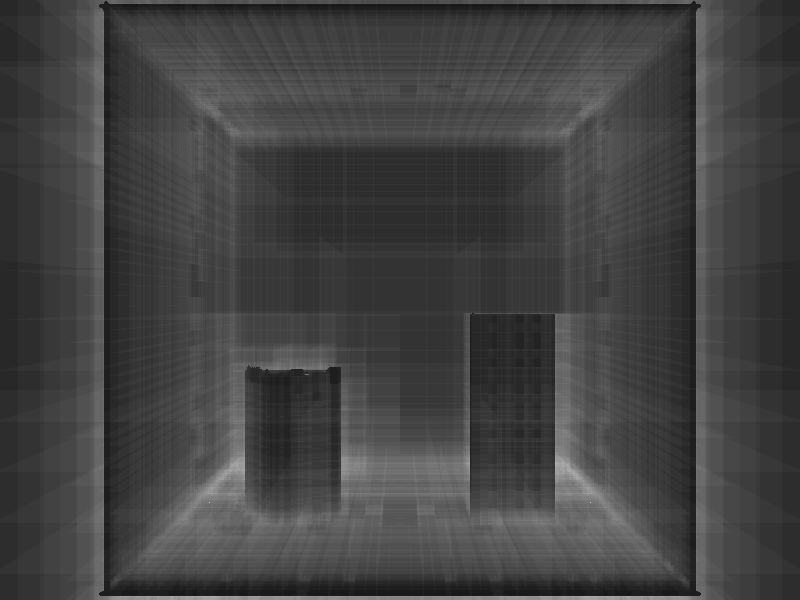
\includegraphics[width=100mm]{img/testing.png}
    \caption{Zoomed image showing PCB extension (left) and Monte Carlo (right.)}
    \label{fig:testing}
\end{figure}


%------------------------------------------------------------%
\section{Adding Scatter-In}
\label{scatterin_sec}
After adding lvoxels to our octree structure and evaluation algorithm, the only modifications necessary for scatter-in are to the volume rendering equation.  

Recall that to model lighting for a volume, in-scattering requires integrating over all directions.  Casting Monte Carlo sample rays through the volume and into the scene would be computationally expensive.  Instead, for each sample we send out rays into the point cloud, iterating through a much less dense dataset.  This helps us replace expensive $S(\textup{p, w})$ evaluations with traversals into the octree.  The two main differences between sampling scattered light within a volume and evaluating the irradiance on a surface are 1) the distribution function, which is based on the volume's phase function, and 2) the samples are distributed over a sphere rather than a hemisphere.

\begin{figure}[h!]
    \centering
    \includegraphics[width=80mm]{img/diag/scatter_in.pdf}
    \captionfonts
    \caption{Comparison of the PCB extension (left) and traditional Monte Carlo results (right.)}
    \label{fig:scatter_in}
\end{figure}


%==============================================================================%
\chapter{Results}

\begin{figure}[h!]
\centering
    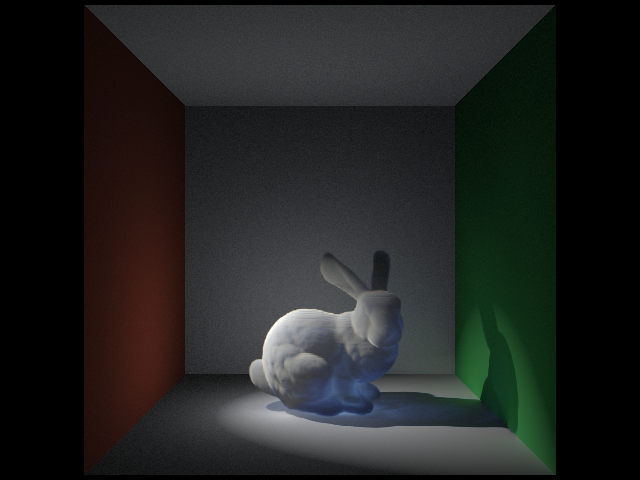
\includegraphics[width=60mm]{img/bunny_spot/spot_left.png}
    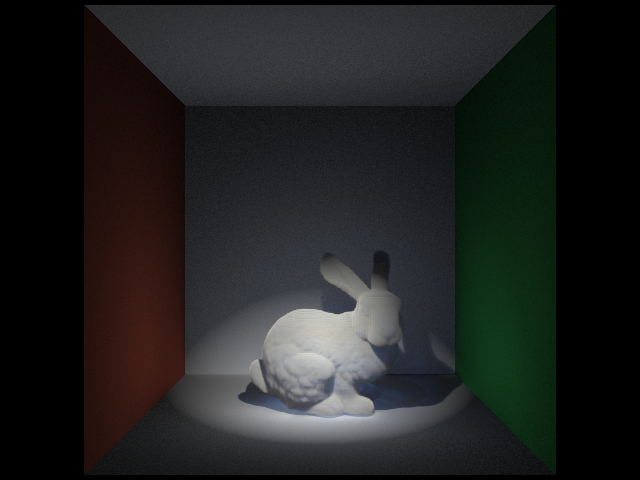
\includegraphics[width=60mm]{img/bunny_spot/spot_front.png}

    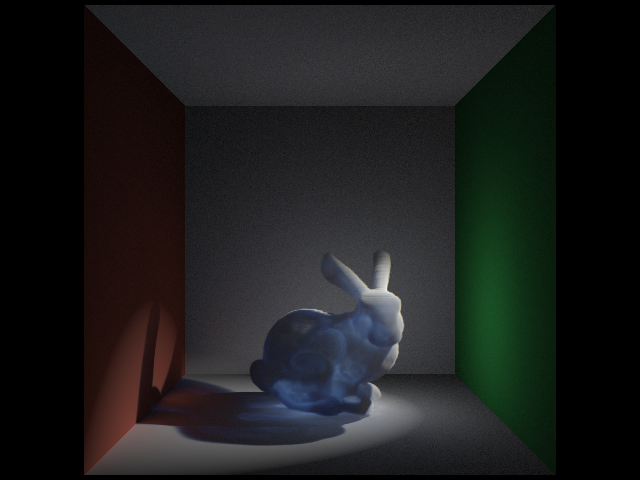
\includegraphics[width=60mm]{img/bunny_spot/spot_right.png}
    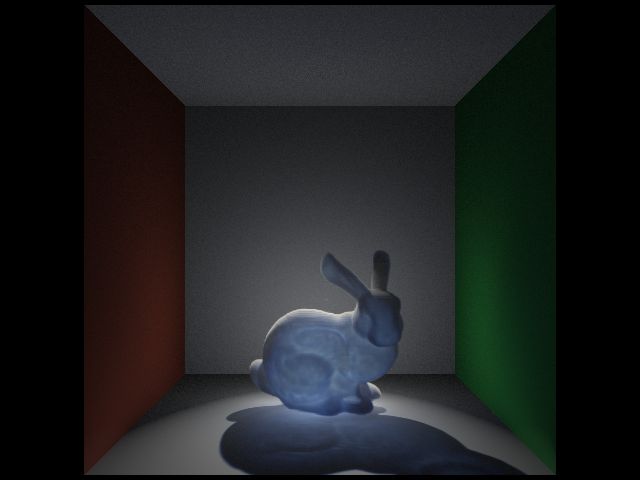
\includegraphics[width=60mm]{img/bunny_spot/spot_behind.png}
    \captionfonts
    \caption{Comparison of the PCB extension (left) and traditional Monte Carlo results (right.)}
\end{figure}

Our algorithm is able to achieve realistic lighting effects for scenes that include volumetric elements using our lvoxel representation with a point-based color bleeding approach to global illumination.
The following test cases were run on a commodity-class Intel i5 3 GHz machine with 4 Gb of RAM.  Because of the disparity between academic-level versus production-class ray tracer implementations, we tested and compared our results against a naive implementation of Monte Carlo global illumination not using the point cloud representation.  We then compared the resulting images and the time it took to render each.  Our algorithm is able to achieve a small difference between images and an increase in efficiency measured in time to render.

The scene tested involved a 60,000 triangle Sponza Atrium including only vertex and normal information for simplicity.  The CT scan data of the Stanford Bunny was used in order to test scatter in/out contributions by complex participating media.
Figure~\ref{fig:compare} shows the bunny and Sponza Atrium showing traditional Monte Carlo scattering.  At first glance these two images are very similar, however there are a number of small artifacts present in the image rendered with the point cloud representation, and the indirect lighting is slightly darker overall.  A closer look at the two results exemplifies the great similarity between the two images, as shown in Figure~\ref{fig:compare_close}.

\begin{figure}[h!]
    \centering
    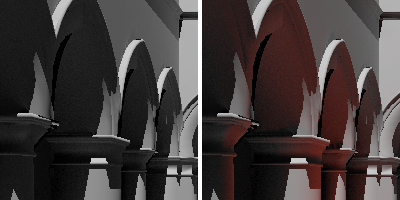
\includegraphics[width=80mm]{img/compare_trad_corrected.png}
    \caption{Zoomed image showing traditional PCB (left) and PCB with extension (right.)  Note the visible color bleeding with our method.}
    \label{fig:compare_trad}
\end{figure}

\begin{figure}[h!]
    \centering
    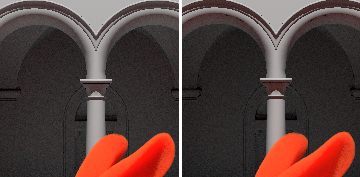
\includegraphics[width=80mm]{img/compare1_corrected.png}
    \caption{Zoomed image showing PCB extension (left) and Monte Carlo (right.)}
    \label{fig:compare_close}
\end{figure}

%------------------------------------------------------------%
\section{Data Comparison}

\begin{center}
\setlength{\tabcolsep}{5pt}
\begin{tabular}{ | l | c | c | c | }
  \hline                       
  Scene & Render Time (s) & Image Delta & Memory Overhead \\
  \hline                  
  Monte Carlo w/o PCB & 3351 sec & NONE & NONE \\
  Traditional PCB & 0385 sec & 11.0\% & 390 Mb (4.0\%) \\
  Extended PCB & 0441 sec & 4.8\% & 395 Mb (4.1\%)  \\
  \hline  
\end{tabular}
\end{center}


%------------------------------------------------------------%
\section{Analysis}

%----------------------------------%
\subsection{Memory}
When using traditional PCB, the real benefit to its surfel representation is shown in more complex scenes.  In the Sponza Atrium, the scene generated over 2.5 million surfels for a 60,000 triangle scene.  Adding volume data to the scene does not add an objectionable amount of data to the point cloud, but for scenes with large volumes the costs could quickly add up without some form of multi-resolution light caching.  In this regard, adding yet another representation of the volumes may be expensive, but not prohibitively so.  Additionally, larger scenes would benefit from this representation, as it would be significantly simpler than the entire scene and can be moved to another system for out-of-core evaluation.

%----------------------------------%
\subsection{Speed}
Even without volume integration, Monte Carlo integration without a lighting representation like PCB is prohibitively slow for even the simplest scenes.  Adding a point cloud representation gave us an impressive speedup.  That speedup was compounded even more when volume scattering was added into the tests, showing a factor of eight speedup for our test scenes.

Even on sparse octrees without volumes, our \textit{front to back} octree traversal method operates at an efficiency of $O\log{n}$ for each node traversal while skipping nodes occluded by surfels, leading to an average performance increase of over 18\%.

%----------------------------------%
\subsection*{Image Quality}
Figure~\ref{fig:compare_trad} compares the non-PCB Monte Carlo image with that of the traditional PCB renders, showing the clear lack of proper in-/out-scattering.  With the extended algorithm, however, the scenes look nearly identical.

We would like to note that there are a number of small artifacts in the PCB renders due to imprecision and incorrect surfel collisions.  It is important to note that, as past papers will attest, such issues are easily overcome and our artifacts are more due to implementation and time constraints than limits on the algorithm itself.

\section{Conclusion}

The addition of the lvoxel paradigm to the already successful point based color bleeding algorithm is shown to be a cost effective method of approximating and evaluating complex scatter functions based on participating media.  The speedups are clear, and the memory footprint is easily manageable.  The ability to evaluate the irradiance at a point in the scene by using only the point cloud representation is a clear win for out-of-core renderers.

%==============================================================================%
\chapter{Future Work}


As mentioned in Christensen's point based color bleeding article, surfels can be modified to ``gather'' light recursively from their position in the point cloud, allowing for simulated multi-bounce lighting.  This would require only a small change to the current algorithm, and would apply to volumes as well to allow very realistic scatter approximations in participating media.

In our tests, all participating media scatters light equally in all directions.  This is rarely the case, as volumes tend to have unique scatter functions.  We can simulate more complex surface scattering functions by creating spherical harmonic representations of the radiance at any specific point in the volume.  Our current implementation supports such an approach, but remains untested.

Typical implementations of the PCB algorithm include rougher estimations (usually in the form of a series of spherical harmonic coefficients) at higher levels in the octree, to be evaluated depending on that node's solid angle to our sample point.  Due to time constraints, we did not implement full multi-resolution representations of each node.  Including LVoxel data in that representation would be a trivial process.

Our ray tracer runs a number of threads to split the image into multiple parts  in order to achieve simple parallelism.  Before the threads are created, however, we generate surfels and lvoxels sequentially.  Due to the nature of our octree implementation, we cannot add elements and still be thread safe, but this would not be a large obstacle.  Scenes like the sponza atrium would run a number of times faster if we were to parallelize our implementation more effectively.


% ------------- End main chapters ----------------------

\clearpage
\bibliography{pcbex}
\bibliographystyle{plain}
%\addcontentsline{toc}{chapter}{Bibliography}



%==============================================================================%


\begin{figure}[h!]
    \centering
    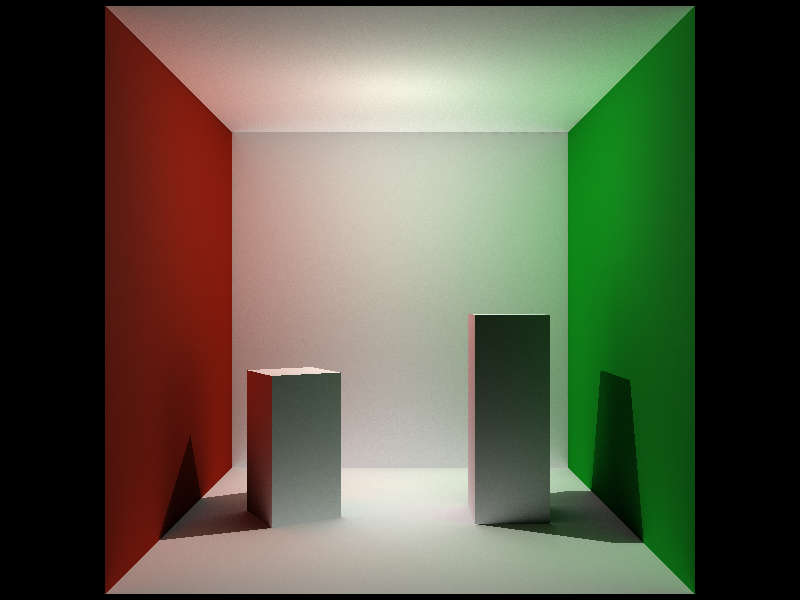
\includegraphics[width=80mm]{img/indirect_box_high.png}
    \caption{Image exemplifying clear out-scattering from Stanford bunny volume.}
\end{figure}

\begin{figure}[h!]
    \centering
    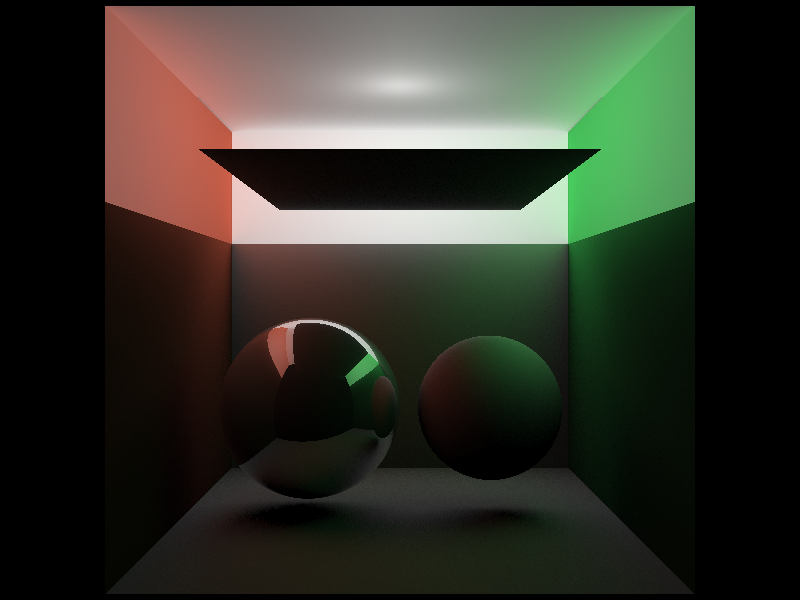
\includegraphics[width=80mm]{img/two_sphere_indir.png}
    \caption{Image exemplifying clear out-scattering from Stanford bunny volume.}
\end{figure}

\begin{figure}[h!]
    \centering
    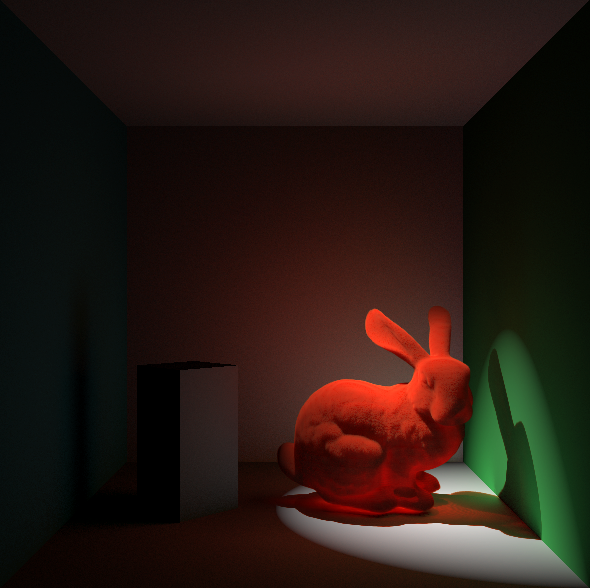
\includegraphics[width=80mm]{img/ketchup_good_corrected.png}
    \caption{Image exemplifying clear out-scattering from Stanford bunny volume.}
\end{figure}

\begin{figure}[h!]
    \centering
    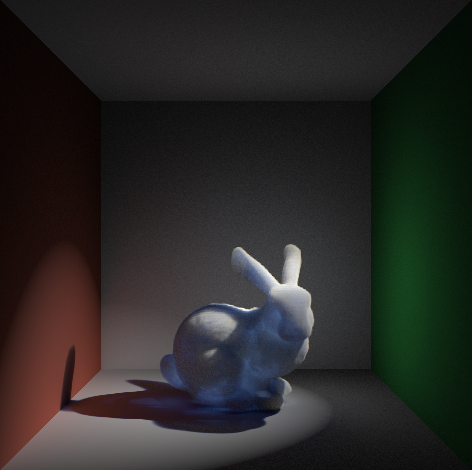
\includegraphics[width=80mm]{img/bunny_spot/spot_right_new.png}
    \caption{Image exemplifying clear color bleeding next to the red wall in the bunny's shadow and correct transmittance through the bunny's hollow form.}
\end{figure}

\begin{figure}[h!]
    \centering
    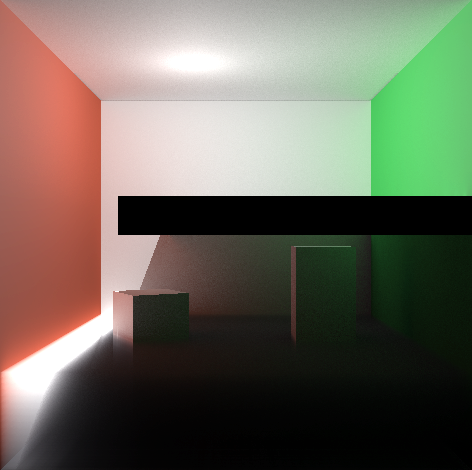
\includegraphics[width=80mm]{img/one_side_corrected.png}
    \caption{The black occluding geometry in the center stops all but the light to the left to enter below.  In and out scattering on the volume and walls is evident.}
\end{figure}



\end{document}
